\section{Sensor Calibration and Computations}
\label{sec:ch3-sensor-calibration}

Sensor calibration converted raw sensor-derived values into engineering units
used by the protection routines. Polynomial calibration was used for the
voltage and current channels because the measured sensor outputs were not
perfectly proportional to the reference instruments over the tested range.
Ordinary least-squares regression estimates coefficients by minimizing the sum
of squared residuals between the measured and fitted values [71]. The
calibration coefficients below were verified from the firmware configuration.
The raw calibration records are retained in Appendix~\ref{app:a},
specifically Tables~\ref{tab:app-a-voltage-calibration},
\ref{tab:app-a-current-calibration}, and
\ref{tab:app-a-temperature-calibration}.

\subsection{Voltage Calibration}
\label{sec:ch3-voltage-calibration}

The voltage calibration setup is shown in
Figure~\ref{fig:ch3-voltage-cal-setup}.
\begin{figure}[H]
  \centering
  
\includegraphics[width=0.90\textwidth]{ch3/figure_3.17.png}
  \caption{Data-collection setup for voltage calibration.}
  \label{fig:ch3-voltage-cal-setup}
\end{figure}

Figure~\ref{fig:ch3-voltage-cal-setup} shows the prototype voltage channel
being compared with reference multimeters while the applied voltage was varied.
The calibration target was the reference RMS voltage, not the uncorrected
sensor output.

The fitted voltage regression is shown in
Figure~\ref{fig:ch3-voltage-regression}.
\begin{figure}[H]
  \centering
  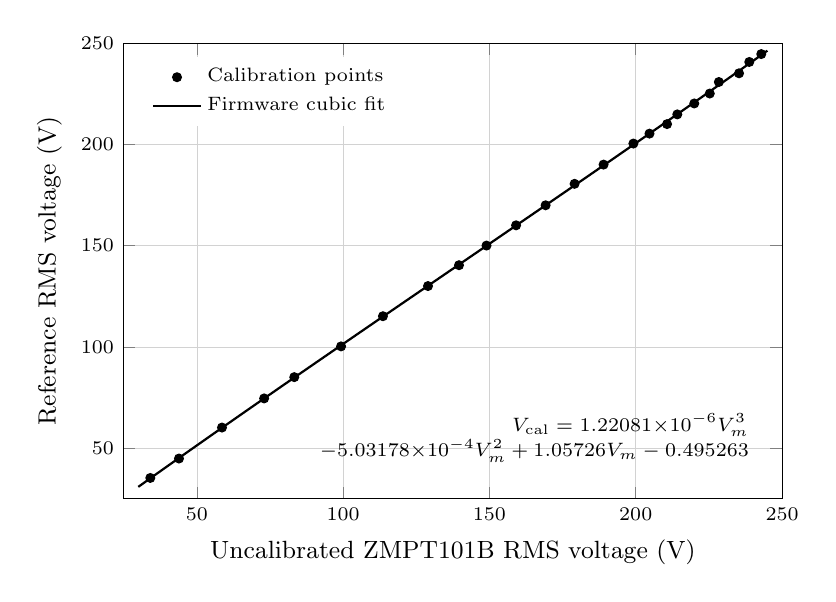
\begin{tikzpicture}
    \begin{axis}[
      width=0.82\textwidth,
      height=2.9in,
      xlabel={Uncalibrated ZMPT101B RMS voltage (V)},
      ylabel={Reference RMS voltage (V)},
      xmin=25,
      xmax=250,
      ymin=25,
      ymax=250,
      grid=major,
      major grid style={line width=0.2pt,draw=gray!35},
      tick label style={font=\scriptsize},
      label style={font=\small},
      legend style={font=\scriptsize,draw=none,at={(0.03,0.97)},anchor=north west},
      legend cell align={left}
    ]
      \addplot[only marks,mark=*,mark size=1.6pt,black] coordinates {
        (34.1,35.2) (43.9,44.79) (58.6,60.1) (73,74.5)
        (83.3,85) (99.3,100.2) (113.6,115.1) (129,130)
        (139.6,140.3) (149,150) (159.1,160) (169.2,169.9)
        (179.1,180.5) (189,190) (199.2,200.4) (204.7,205.3)
        (210.7,210) (214.2,214.8) (220,220.2) (225.3,225.1)
        (228.4,230.8) (235.3,235.1) (238.8,240.7) (242.9,244.6)
      };
      \addlegendentry{Calibration points}
      \addplot[black,thick,domain=30:245,samples=160]
        {1.22081e-6*x^3 - 5.03178e-4*x^2 + 1.05726*x - 0.495263};
      \addlegendentry{Firmware cubic fit}
      \node[anchor=south east,font=\scriptsize,align=right] at (axis cs:242,38)
        {$V_{\mathrm{cal}}=1.22081{\times}10^{-6}V_m^3$\\
         $-5.03178{\times}10^{-4}V_m^2+1.05726V_m-0.495263$};
    \end{axis}
  \end{tikzpicture}
  \caption{Cubic regression for voltage calibration.}
  \label{fig:ch3-voltage-regression}
\end{figure}

Figure~\ref{fig:ch3-voltage-regression} supports the cubic correction used by
the firmware. The implemented voltage calibration is
\begin{equation}
  V_{\mathrm{cal}} =
  1.22081\times10^{-6}V_m^3
  - 5.03178\times10^{-4}V_m^2
  + 1.05726V_m
  - 0.495263 .
  \label{eq:voltage-calibration}
\end{equation}
In (\ref{eq:voltage-calibration}), $V_m$ is the measured RMS voltage before
the cubic correction and $V_{\mathrm{cal}}$ is the calibrated RMS voltage used
for display and voltage protection. The polynomial correction is needed
because threshold decisions such as undervoltage, overvoltage, and
mains-present detection depend on the calibrated value.

\subsection{Current Calibration}
\label{sec:ch3-current-calibration}

The current calibration setup and load combinations are shown in
Figures~\ref{fig:ch3-current-cal-setup} and~\ref{fig:ch3-current-cal-loads}.

\begin{figure}[H]
  \centering
  
\includegraphics[width=0.90\textwidth]{ch3/figure_3.19.png}
  \caption{Data-collection setup for current calibration.}
  \label{fig:ch3-current-cal-setup}
\end{figure}

\begin{figure}[H]
  \centering
  
\includegraphics[width=0.90\textwidth]{ch3/figure_3.20.png}
  \caption{Load setups used for current calibration.}
  \label{fig:ch3-current-cal-loads}
\end{figure}

Figure~\ref{fig:ch3-current-cal-setup} shows the comparison between the
prototype current channel and a reference instrument.
Figure~\ref{fig:ch3-current-cal-loads} shows the different resistive and
appliance loads used to span the current range needed for overload and
arc-feature testing.

The fitted current regression is shown in
Figure~\ref{fig:ch3-current-regression}.
\begin{figure}[H]
  \centering
  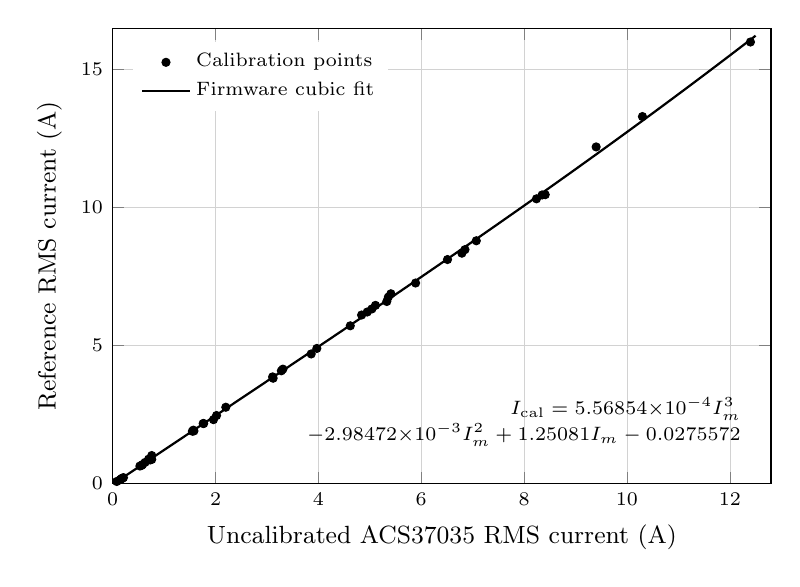
\begin{tikzpicture}
    \begin{axis}[
      width=0.82\textwidth,
      height=2.9in,
      xlabel={Uncalibrated ACS37035 RMS current (A)},
      ylabel={Reference RMS current (A)},
      xmin=0,
      xmax=12.8,
      ymin=0,
      ymax=16.5,
      grid=major,
      major grid style={line width=0.2pt,draw=gray!35},
      tick label style={font=\scriptsize},
      label style={font=\small},
      legend style={font=\scriptsize,draw=none,at={(0.03,0.97)},anchor=north west},
      legend cell align={left}
    ]
      \addplot[only marks,mark=*,mark size=1.45pt,black] coordinates {
        (0.08,0.08) (0.15,0.15) (0.17,0.18) (0.19,0.2)
        (0.21,0.22) (0.53,0.64) (0.56,0.66) (0.58,0.69)
        (0.63,0.77) (0.73,0.86) (0.76,0.88) (0.7,0.89)
        (0.76,1.02) (1.55,1.9) (1.58,1.91) (1.57,1.94)
        (1.76,2.18) (1.77,2.18) (1.96,2.32) (2.02,2.47)
        (2.2,2.77) (3.12,3.82) (3.11,3.87) (3.28,4.09)
        (3.31,4.15) (3.86,4.7) (3.97,4.9) (5.89,7.27)
        (4.62,5.72) (4.84,6.11) (4.95,6.22) (5.04,6.33)
        (5.11,6.46) (5.33,6.6) (5.36,6.76) (5.41,6.88)
        (6.51,8.12) (6.79,8.35) (6.85,8.48) (7.07,8.8)
        (8.24,10.32) (8.35,10.46) (8.41,10.47) (9.4,12.2)
        (10.3,13.3) (12.4,16)
      };
      \addlegendentry{Calibration points}
      \addplot[black,thick,domain=0:12.5,samples=160]
        {5.56854e-4*x^3 - 2.98472e-3*x^2 + 1.25081*x - 0.0275572};
      \addlegendentry{Firmware cubic fit}
      \node[anchor=south east,font=\scriptsize,align=right] at (axis cs:12.4,1.0)
        {$I_{\mathrm{cal}}=5.56854{\times}10^{-4}I_m^3$\\
         $-2.98472{\times}10^{-3}I_m^2+1.25081I_m-0.0275572$};
    \end{axis}
  \end{tikzpicture}
  \caption{Cubic regression for current calibration.}
  \label{fig:ch3-current-regression}
\end{figure}

The implemented current calibration is
\begin{equation}
  I_{\mathrm{cal}} =
  5.56854\times10^{-4}I_m^3
  - 2.98472\times10^{-3}I_m^2
  + 1.25081I_m
  - 0.0275572 .
  \label{eq:current-calibration}
\end{equation}
In (\ref{eq:current-calibration}), $I_m$ is the measured RMS current before
the cubic correction and $I_{\mathrm{cal}}$ is the calibrated RMS current used
by the overload logic, socket-temperature model, and waveform-feature
extractor. Negative fitted values are clamped to zero in firmware.

The device temperature measurement calibration setup is shown in
Figure~\ref{fig:ch3-ntc-cal-setup}.

\subsection{Device Temperature Measurement Calibration}
\label{sec:ch3-device-temperature-calibration}

\begin{figure}[H]
  \centering
  
\includegraphics[width=0.85\textwidth]{ch3/figure_3.22.jpg}
  \caption{Data-collection setup for device temperature measurement calibration.}
  \label{fig:ch3-ntc-cal-setup}
\end{figure}

Figure~\ref{fig:ch3-ntc-cal-setup} shows the external thermistor measurement
being compared with a reference temperature measurement. Thermistor placement
is important because an external sensor can lag or under-read the hottest
contact point inside a degraded socket [27], [29], [30]. The acquired
temperature-resistance calibration points are listed in
Table~\ref{tab:app-a-temperature-calibration}.

The firmware computes the NTC resistance from the voltage-divider output:
\begin{equation}
  R_{\mathrm{NTC}} =
  \frac{V_{\mathrm{NTC}}R_D}{V_{\mathrm{CC}} - V_{\mathrm{NTC}}}.
  \label{eq:ntc-resistance}
\end{equation}
In (\ref{eq:ntc-resistance}), $V_{\mathrm{NTC}}$ is the measured divider
voltage, $R_D=3.3\mathrm{k}\Omega$ is the fixed divider resistor, and
$V_{\mathrm{CC}}=3.3\mathrm{V}$ is the divider supply. The resistance is then
converted to temperature with the Beta equation:
\begin{equation}
  T_{\mathrm{NTC}} =
  \left[
  \frac{1}{T_0} +
  \frac{1}{\beta}\ln\left(\frac{R_{\mathrm{NTC}}}{R_0}\right)
  \right]^{-1}
  - 273.15 .
  \label{eq:ntc-beta}
\end{equation}
In (\ref{eq:ntc-beta}), $T_{\mathrm{NTC}}$ is in degrees Celsius, $T_0 =
298.15\mathrm{K}$, $R_0=10\mathrm{k}\Omega$, and $\beta=4050$. The
computed temperature is clamped from $-20\degreeC$ to $125\degreeC$ and
filtered with a 3s time constant in the temperature-sensing routine.

\section{Socket-Heating Temperature Models}
\label{sec:ch3-socket-heating-models}

The socket-heating computation uses two related models. The first is the
expected normal socket temperature, which estimates the socket temperature
expected under healthy contact behavior. The second is the estimated socket
temperature, which is the protection-facing compensated value intended to
respond to degraded-contact heating and external device temperature under-reading. This
separation is necessary because a raw external thermistor does not directly
measure the internal contact hotspot [30], [46], [47].

\subsection{Expected Normal Temperature Model}
\label{sec:ch3-expected-normal-temperature}

The firmware first decides whether the load is active:
\begin{equation}
  L =
  \begin{cases}
  1, & \text{if mains is present and } I_{\mathrm{rms}}\geq 0.35\mathrm{A},\\
  0, & \text{otherwise}.
  \end{cases}
  \label{eq:load-active}
\end{equation}
In (\ref{eq:load-active}), $L$ is the load-active flag and
$I_{\mathrm{rms}}$ is the calibrated RMS current. When $L=0$, the current
dependent thermal rise is forced toward zero.

The current-dependent shape term is
\begin{equation}
  s_I =
  \left[
  \mathrm{clamp}\left(\frac{I_{\mathrm{rms}}}{12.0},\,0,\,1.25\right)
  \right]^2 .
  \label{eq:thermal-current-shape}
\end{equation}
In (\ref{eq:thermal-current-shape}), $s_I$ is the normalized squared current
term. The 12.0A denominator and 1.25 clamp are firmware constants. The square
term reflects that heat generation associated with resistive loss rises with
current squared.

The ambient or baseline term is tracked from the device temperature measurement only when the
load is off or the current is below 0.18A:
\begin{equation}
  T_a[k] = T_a[k-1] + \alpha_a\left(T_{\mathrm{NTC}}[k] - T_a[k-1]\right),
  \qquad
  \alpha_a = \frac{\Delta t}{240\mathrm{s}} .
  \label{eq:thermal-ambient}
\end{equation}
In (\ref{eq:thermal-ambient}), $T_a$ is the inferred ambient or baseline
temperature, $\Delta t$ is the elapsed firmware update time, and
$T_{\mathrm{NTC}}$ is the measured thermistor temperature. The 240s time
constant prevents the baseline from following short-term load heating.

The target normal rise is
\begin{equation}
  \Delta T_{\mathrm{normal,target}} =
  \begin{cases}
  0.20 + 12.0s_I, & L=1,\\
  0, & L=0 .
  \end{cases}
  \label{eq:normal-target-rise}
\end{equation}
In (\ref{eq:normal-target-rise}), $0.20\degreeC$ is the normal base rise and
$12.0\degreeC$ is the normal current-rise gain. The fitted-gain source file
was not present in the codebase; the least-squares derivation should therefore
be checked against Appendix~\ref{app:c} or the original characterization
worksheet.

The firmware filters this target with separate heating and cooling time
constants:
\begin{equation}
  \Delta T_{\mathrm{normal}}[k]
  =
  \Delta T_{\mathrm{normal}}[k-1]
  +
  \alpha_n\left(
  \Delta T_{\mathrm{normal,target}}[k] -
  \Delta T_{\mathrm{normal}}[k-1]\right).
  \label{eq:normal-rise-filter}
\end{equation}
In (\ref{eq:normal-rise-filter}), $\alpha_n=\Delta t/900\mathrm{s}$ when the
target rise is increasing and $\alpha_n=\Delta t/1800\mathrm{s}$ when the
target rise is decreasing. These time constants represent the slower thermal
response of the socket compared with the electrical measurements.

The expected normal socket temperature is then
\begin{equation}
  T_{\mathrm{normal,exp}} =
  \mathrm{clamp}
  \left(T_a + \Delta T_{\mathrm{normal}},\, -20,\,125\right).
  \label{eq:expected-normal-socket}
\end{equation}
In (\ref{eq:expected-normal-socket}), $T_{\mathrm{normal,exp}}$ is the
baseline or normal thermal estimate. It represents what the socket temperature
should be under expected contact behavior for the measured current history.

\subsection{Estimated Socket Temperature Model}
\label{sec:ch3-estimated-socket-temperature-model}

The measured device temperature value is compensated directly:
\begin{equation}
  T_{\mathrm{comp}} =
  \mathrm{clamp}
  \left(T_{\mathrm{NTC}} + \Delta T_{\mathrm{meas}},\, -20,\,125\right),
  \qquad
  \Delta T_{\mathrm{meas}} =
  \begin{cases}
  0.30 + 1.20s_I, & L=1,\\
  0, & L=0 .
  \end{cases}
  \label{eq:measured-compensation}
\end{equation}
In (\ref{eq:measured-compensation}), $T_{\mathrm{comp}}$ is the compensated
thermistor-based estimate, $0.30\degreeC$ is the measured base delta, and
$1.20\degreeC$ is the measured current gain. These constants were verified
from the firmware configuration; their original least-squares fitting
worksheet must be verified manually if the derivation is required in the final
defense copy.

Finally, the protection-facing socket estimate is
\begin{equation}
  T_{\mathrm{socket,est}} =
  \mathrm{clamp}
  \left(
  \max\left(T_{\mathrm{comp}}, T_{\mathrm{normal,exp}}\right),
  -20,
  125
  \right).
  \label{eq:estimated-socket-temp}
\end{equation}
In (\ref{eq:estimated-socket-temp}), $T_{\mathrm{socket,est}}$ is the
estimated socket temperature used by the protection manager. The maximum
operation makes the estimator conservative: it does not allow the compensated
device temperature estimate to fall below the expected normal socket estimate when load
current indicates that some heating should be present.

The verified thermal constants are summarized in
Table~\ref{tab:ch3-thermal-constants}.
\begin{table}[H]
  \centering
  \caption{Socket-heating constants verified from firmware}
  \label{tab:ch3-thermal-constants}
  \begin{tabular}{p{0.40\textwidth}p{0.20\textwidth}p{0.30\textwidth}}
    \toprule
    \textbf{Constant} & \textbf{Value} & \textbf{Function} \\
    \midrule
    Load-on current threshold & 0.35A & Enables current-dependent heating model \\
    Ambient tracking current limit & 0.18A & Allows baseline tracking only at very low load \\
    Ambient time constant & 240s & Slow baseline update \\
    Normal reference current & 12.0A & Denominator for current-shape term \\
    Normal base rise & 0.20°C & Minimum expected rise when load is active \\
    Normal current gain & 12.0°C & Expected normal heating gain \\
    Current-ratio clamp & 1.25 & Limits current-shape term \\
    Heating time constant & 900s & Rise filter for normal estimate \\
    Cooling time constant & 1800s & Fall filter for normal estimate \\
    Measured base delta & 0.30°C & Direct thermistor compensation offset \\
    Measured current gain & 1.20°C & Direct thermistor compensation gain \\
    Estimated-temperature trip threshold & 40.0°C & Thermal relay trip threshold \\
    Thermal warning and clear thresholds & 39.0°C / 38.6°C & Warning hysteresis \\
    \bottomrule
  \end{tabular}
\end{table}

Table~\ref{tab:ch3-thermal-constants} distinguishes the thermal estimator from
the warning and trip thresholds. The estimator produces
$T_{\mathrm{socket,est}}$, while the protection manager decides warning and
relay action from that estimate.

\subsection{Least-Squares Gain and Regression Derivation}
\label{sec:ch3-thermal-least-squares}

The intended calibration path for the socket-heating constants is to compare
the device temperature measurement and reference terminal readings against ambient, then
fit the compensation terms from the characterization records. For a gain-only
rise model, the least-squares gain is
\begin{equation}
  k =
  \frac{\sum_i x_i y_i}{\sum_i x_i^2},
  \label{eq:thermal-gain-fit}
\end{equation}
where $x_i$ is the predictor rise above ambient, such as device temperature measurement
rise or current-shaped rise, and $y_i$ is the reference terminal rise above
ambient. When an offset is required, the corresponding linear model is
\begin{equation}
  \Delta T_{\mathrm{ref}} =
  a\Delta T_{\mathrm{device}} + b .
  \label{eq:thermal-linear-fit}
\end{equation}
In (\ref{eq:thermal-linear-fit}), $\Delta T_{\mathrm{ref}}$ is the infrared
thermometer or terminal-contact rise and $\Delta T_{\mathrm{device}}$ is the
external thermistor rise. If time lag is evident, the time series should be
aligned before fitting. The source worksheet used to choose the firmware
constants was not present in the repository, so the constants in
Table~\ref{tab:ch3-thermal-constants} are reported as verified firmware
constants and should be recomputed from Appendix~\ref{app:c} or the original
worksheet before final defense submission.

\subsection{Firmware Implementation of Constants}
\label{sec:ch3-thermal-firmware-constants}

As an example, consider a load-active frame at $I_{\mathrm{rms}}=9.04\mathrm{A}$.
The current-shape term in (\ref{eq:thermal-current-shape}) is
\[
  s_I=\left(\frac{9.04}{12.0}\right)^2=0.568 .
\]
The direct thermistor-compensation rise in
(\ref{eq:measured-compensation}) is therefore
$0.30+1.20(0.568)=0.982\degreeC$. If the device temperature measurement for that
frame is $38.2\degreeC$, the direct compensated estimate is
$T_{\mathrm{comp}}=39.18\degreeC$ before the final maximum operation. For the
same current, the normal target rise in (\ref{eq:normal-target-rise}) is
$0.20+12.0(0.568)=7.02\degreeC$. The final protection-facing estimate still
depends on the filtered normal-rise state and inferred ambient term, which is
why the method evaluates a thermal history rather than only a single
instantaneous current and device temperature reading.
